\documentclass[12pt,twoside]{article}

% Things that are not loaded by the package, though these might be
% generally useful.
\usepackage{natbib}
\usepackage{graphicx}
\setcounter{secnumdepth}{0}

\usepackage{amsthm}

\renewcommand\thefigure{S.\arabic{figure}}
\renewcommand\thetable{S.\arabic{table}}

% Load the package first - should sort everything out...
\usepackage{suppmat}

% ...and then we add some metadata
\titleprefix{Supplemental Material}
\runninghead{Y fuse?}
\title{Y fuse? Sex chromosome fusions in fishes and reptiles}
\author{Jun Kitano$^1$, Matthew W. Pennell$^2$, Mark Kirkpatrick$^3$,\\ Sarah P. Otto$^4$, Jana C. Vamosi$^5$, \& Catherine L. Peichel$^6$}
\address{
1& Ecological Genetics Laboratory, National Institute of Genetics, Mishima, Shizuoka 411-8540, Japan\\
2& Institute for Bioinformatics and Evolutionary Studies, University of Idaho, Moscow, ID 83844, USA\\
3& Department of Integrative Biology, University of Texas, Austin, TX 78712, USA\\
4& Department of Zoology, University of British Columbia, Vancouver, BC V6J 3S7, Canada\\
5& Department of Biological Sciences, University of Calgary, Calgary, AB T2N 1N4, Canada\\
6& Divison of Human Biology, Fred Hutchinson Cancer Research Center, Seattle, WA 98109, USA\\}
\emailaddress{\email{jkitano@lab.nig.ac.jp}}
\date{}

\begin{document}

\maketitle

\section{Details of phylogenetic analyses}

To investigate the relative rates of different types of fusions across our two focal groups--teleost fishes and squamate reptiles--we fit multiple phylogenetic models to our karyotype dataset. We first matched the available karyotype data to the fish \citep{Rabosky2013} and squamate \citep{squamatetree, PyronBurbrink2014} phylogenies (using an approximate matching algorithm described in the main text). This resulted in phylogenetic comparative datasets containing 163 species of fish and 261 squamate species.  We conducted two separate types of analyses on both groups. First, we examined differences between XY and ZW systems; here, we treat X-autosome and Y-autosome fusions as equivalent (and likewise, Z-autosome and W-autosome fusions). Results from this first analysis are presented in the main text. Second, we investigated autosomal fusion rates for all types of sex chromosomes individually (i.e., Y, X, W, and Z autosome fusions). While the second analysis provides more detailed resolution, some of the states are rarely observed (and in some cases, not at all). All analyses were performed using the R package \textsc{diversitree} \citep{FitzJohn2012}, and code to reproduce all results can be found at \texttt{https://github.com/mwpennell/fuse/analysis}. 

\subsection{Fusion rates in XY vs. ZW systems}

Using a Markov model \citep{Pagel1994}, we considered transitions among the following states:
\begin{itemize}
\item $XY$: Male heterogametic unfused
\item $XY_F$: Male heterogametic fused (XXY or XYY)
\item $ZW$: Female heterogametic unfused
\item $ZW_F$: Female heterogametic fused (ZZW or ZWW)
\end{itemize}
allowing transitions between all states with $q_{A.B}$ representing the transition rate between states $A$ and $B$. We then used likelihood ratio tests to restrict the model in order to improve our ability to estimate the parameters of interest. 

We first imposed the biologically reasonable constraint that prior to becoming $XY_F$ (or $ZW_F$), a lineage must first be $XY$ (or $ZW$); e.g., the transition rate from female heterogametic unfused to male heterogametic fused $q_{ZW.XY_F}$ would be zero. These restrictions did not lead to a significant decline in likelihood for either squamates or fish and was accepted.

Next, we proposed a model in which the rate of switching the heterogametic sex, going from a XY to a ZW system and \emph{vice versa}, did not depend on whether the lineage contained a fused sex chromosome or not (e.g., $q_{XY_F.ZW} = q_{XY.ZW}$). In both fish and squamtes, this restriction was acceptable.

In the next step, we proposed a model in which the rate of chromosomal fission, going from a fused sex chromosome system to an unfused system of the same type, was the same for XY and ZW systems. In fish, a likelihood ratio test favored the more restricted model, whereas in squamates, the more general model (where $q_{XY_F.XY} \neq q_{ZW_F.ZW}$) was favored ($p=\text{0.012}$). The support for the more general model in squamates stems from the scarcity of ZW fusions in the data; there is little information to reliably estimate the transition rate from fused female heterogametic to unfused female heterogametic ($q_{ZW_F.ZW}$) using maximum likelihood (see below). We therefore took slightly different approaches when analyzing the two clades.

For fish, we compared the resulting model ($q_{XY_F.XY} = q_{ZW_F.ZW}, q_{ZW.XY_F}=q_{XY.ZW_F}=\text{0}, q_{XY_F.ZW}=q_{XY_Z.ZW}, q_{ZW_F.XY}=q_{ZW.XY}$) to an even more reduced model in which the XY and ZW fusion rates were set to be equal ($q_{XY.XY_F}=q_{ZW.ZW_F}$). We found the rate difference to be highly significant ($p=\text{0.014}$) using a likelihood ratio test. To better accomodate uncertainty in the estimate, we ran a Bayesian analysis (described in the text), and this too supported our conclusion that XY fusions occur at a higher rate than ZW fusions (98.6\% of the posterior probability supported this and the 95\% credibility interval for the difference in rates did not overlap with zero; Figure 4 in the main text).

For the squamate data, we took two approaches. First, we assumed that the `equal fission rates model' was indeed reasonable and performed the same analysis as in fish. Using a likelihood ratio test, the difference in fusion rates for XY and ZW was found to be highly significant ($p=\text{0.003}$). The same was true for the Bayesian analysis (99.9\% of the posterior probability distribution supported this conclusion; Figure 4 in the main text). Second, we used a Bayesian MCMC to fit a model in which the fission rate $q_{ZW_F.ZW}$ was estimated independently of $q_{XY_F.XY}$. For this model the support for the difference between XY and ZW fusion rates was not as strong (92.0\% of the posterior probability supported $q_{XY.XY_F} > q_{ZW.ZW_F}$; Figure \ref{fig:squa-dif}).

\begin{figure}[p]
\centering
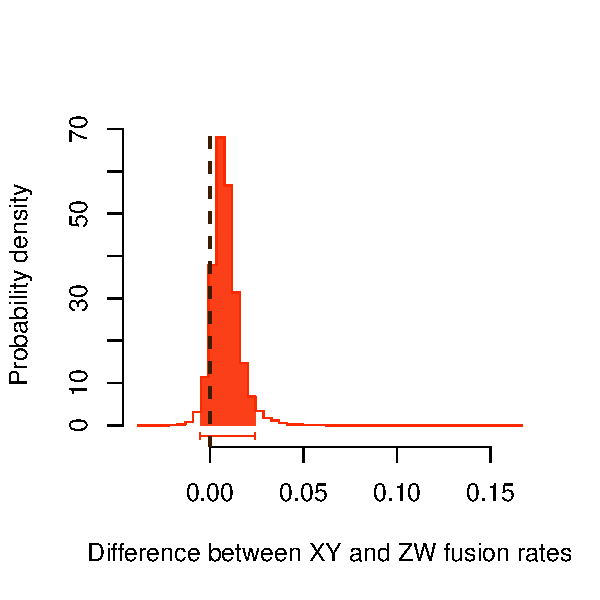
\includegraphics[scale=1.25]{figs/karyotype-fusion-squa-6par}
\caption{Posterior estimate of the rate difference between XY and ZW fusions ($q_{XY.XY_F} - q_{ZW.ZW_F}$) in squamate reptiles when we allow the fission rates $q_{XY_F.XY}$ and $q_{ZW_F.ZW}$ to differ.}
\label{fig:squa-dif}
\end{figure}

As mentioned above, the squamate data contain very little information about fission rates, especially from $ZW_F$ to $ZW$. The likelihood approach has difficulty distinguishing between two explanations for the lack of fused ZW chromosomes: rare ZW fusions or common ZW fissions. Nevertheless, there is a strong signal that ZW fusions should be less common, which we confirmed by considereing residency times $t_R$. For XY fusions,
\begin{equation}
t_{R,XY_F} = \frac{q_{XY.XY_F}}{(q_{XY.XY_F} + q_{XY_F.XY})}
\end{equation}
and for ZW fusions
\begin{equation}
t_{R,ZW_F} = \frac{q_{ZW.ZW_F}}{(q_{ZW.ZW_F} + q_{ZW_F.ZW})}
\end{equation}
Using a Bayesian analysis, we found very strong support for the residency time being greater for XY fusions than ZW fusions (99.8\% of the posterior probability supported $t_{R,XY_F} > t_{R,ZW_F}$; Figure \ref{fig:squa-resid}). In the absence of direct information about fission rates for fused ZW chromosomes, we conclude that the data is more parsimoniously explained by rare ZW fusions, while acknowledging that rapid ZW fission rates may also explain the data for squamates.

\begin{figure}[p]
\centering
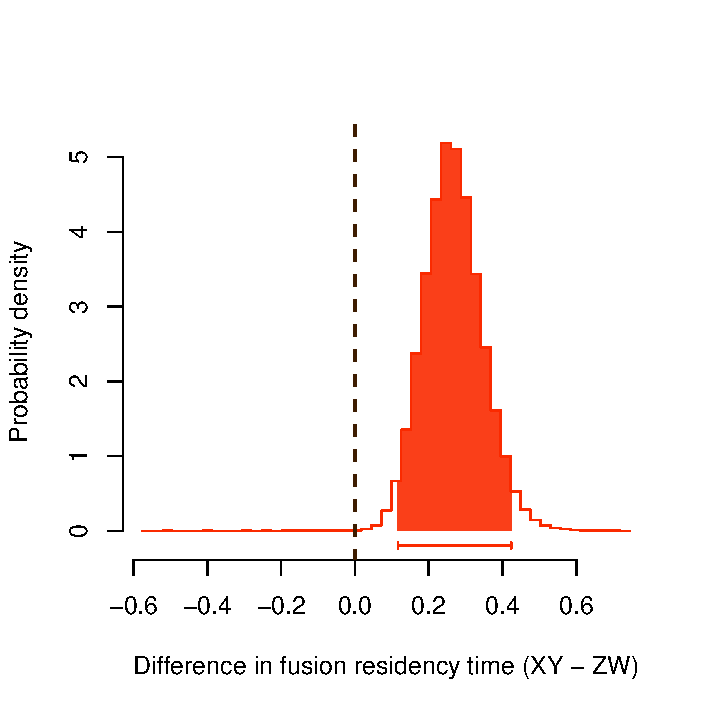
\includegraphics[scale=1.1]{figs/karyotype-residency-squa-6par}
\caption{Posterior estimate of the difference in residency time between XY and ZW fusions (i.e., $q_{R,XY_F} - q_{R,ZW_F}$) in squamate reptiles.}
\label{fig:squa-resid}
\end{figure}


\subsection{Comparing fusion rates between chromosomes} 

Rather than classifying the states as male/female heterogametic unfused/fused, we separated out the different types of fusions (e.g., classifying X-autosome [XA] and Y-autosome [YA] fusions as different states). This allowed us to assess whether the patterns we observed were driven by an overabundance of autosomal fusions with the Y chromosome. After matching the data to the tree, we did not have any records of WA fusions in fish while in squamates, XA fusions were absent. We thus considered models with only three fused states (for fish: XA, YA, and ZA; for squamates: YA, WA, and ZA)

For both the fish and the squamates, we again restricted the model via a nested series of likelihood ratio tests. For both clades, we found it to be statistically justifiable to assume that: a) transitions from one fused state directly to another fused state were impossible; b) prior to becoming fused, a lineage had to be in the corresponding unfused state; and c) fission rates were constrained to be equal. This allowed us to reliably evaluate whether the fusion rates differed by chromosome.

For the fish, using likelihood ratio tests, we found YA fusions to be significantly higher than XA fusions ($p=\text{0.016}$) and ZA fusions ($p=\text{0.035}$), but that XA and ZA fusion rates were not significantly different ($p=\text{0.658}$). Again, WA fusions did not exist in the fish analysis so we could not compare them to other classes. We then performed a Bayesian MCMC analysis to gain a better estimate of the relevant parameters. For the purposes of this analysis, we fixed XA and ZA fusions to occur at the same rate and then compared this rate to that for YA fusion. We found that YA fusions occur at a much higher rate than XA/ZA fusions (Figure \ref{fig:fish-ind}; 99.5\% of the posterior distribution supported this conclusion).

\begin{figure}[p]
\centering
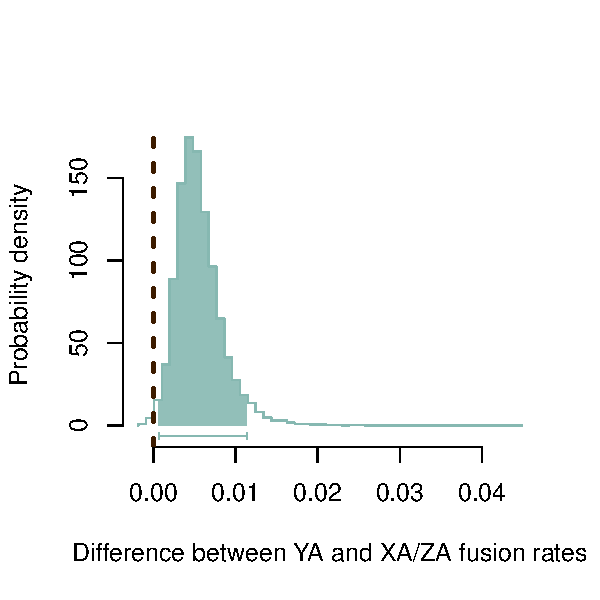
\includegraphics[scale=1.25]{figs/chromosome-fusion-fish}
\caption{Posterior estimate of the rate difference between YA and XA/ZA fusions in fish. When the estimate is greater than zero, this means that the YA fusion rates are higher than those of the other chromosomes}
\label{fig:fish-ind}
\end{figure}

For the squamate analysis, YA fusions also occured at a higher rate than WA fusions ($p<\text{0.001}$) and ZA fusions ($p<\text{0.001}$). WA and ZA fusions rates were not significantly different from one another ($p\approx \text{1}$). As with the fish, for the Bayesian analysis we set WA and ZA fusion rates to be equal and estimated the difference between YA fusions and other type of fusions. 99.9\% of the posterior probability distribution supported YA fusions occuring at a higher rate than fusions on other chromosomes (Figure \ref{fig:squa-ind}). 

Taken together, these results strongly suggest that the difference between XY and ZW fusion rates is driven almost entirely by the very high rates of autosomal fusions involving the Y chromosome relative to the other sex chromosomes.

\begin{figure}[p]
\centering
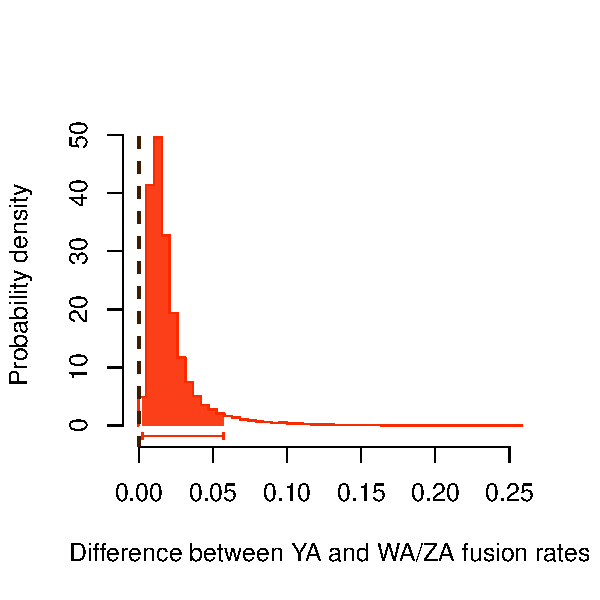
\includegraphics[scale=1.25]{figs/chromosome-fusion-squa}
\caption{Posterior estimate of the rate difference between YA and WA/ZA fusions in squamate reptiles. When the estimate is greater than zero, this means that the YA fusion rates are higher than those of the other chromosomes}
\label{fig:squa-ind}
\end{figure}

\clearpage
\bibliographystyle{sysbio}
\bibliography{suppmat.bib}

\end{document}
